\documentclass{standalone}
\usepackage{tikz}
\usetikzlibrary{patterns, positioning}
\usepackage[sfdefault]{ClearSans} %% option 'sfdefault' activates Clear Sans as the default text font
\usepackage[T1]{fontenc}

\begin{document}
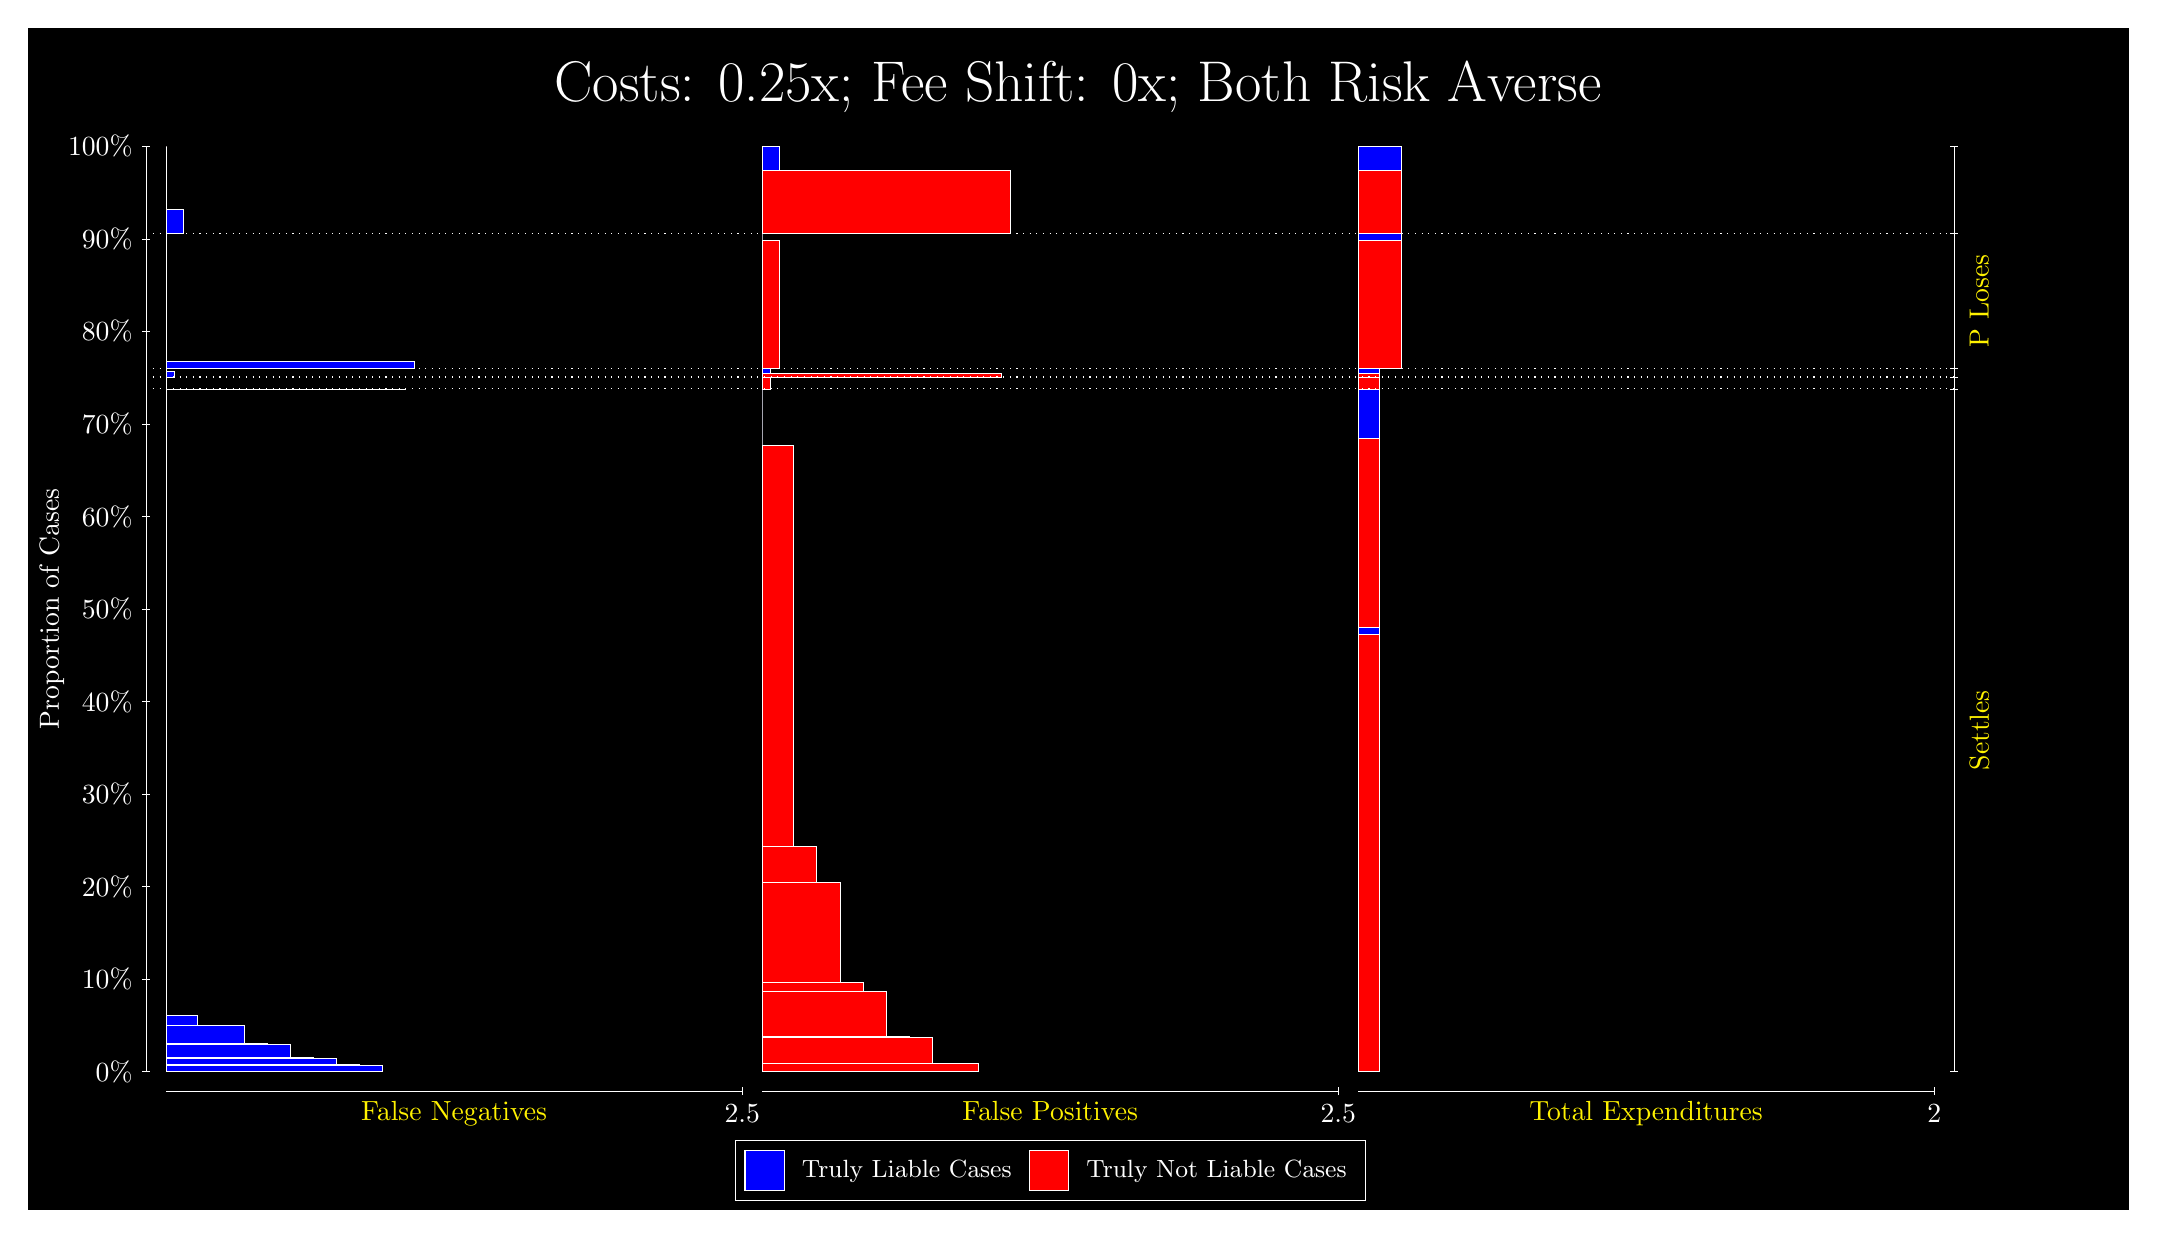
\begin{tikzpicture}
\draw[fill=black] (0,0) rectangle (26.667,15);
\draw[text=white] (0,13.5) rectangle (26.667,15) node[midway] {\huge Costs: 0.25x; Fee Shift: 0x; Both Risk Averse};
\draw[white, very thin] (1.5,1.75) -- (1.5,13.5);
\node[rotate=90, text=white, anchor=center] at (0.3, 7.625) {Proportion of Cases};
\draw[white, very thin] (1.45,1.75) -- (1.55,1.75);
\node[text=white, anchor=east] at (1.45, 1.75) {0\%};
\draw[white, very thin] (1.45,2.925) -- (1.55,2.925);
\node[text=white, anchor=east] at (1.45, 2.925) {10\%};
\draw[white, very thin] (1.45,4.1) -- (1.55,4.1);
\node[text=white, anchor=east] at (1.45, 4.1) {20\%};
\draw[white, very thin] (1.45,5.275) -- (1.55,5.275);
\node[text=white, anchor=east] at (1.45, 5.275) {30\%};
\draw[white, very thin] (1.45,6.45) -- (1.55,6.45);
\node[text=white, anchor=east] at (1.45, 6.45) {40\%};
\draw[white, very thin] (1.45,7.625) -- (1.55,7.625);
\node[text=white, anchor=east] at (1.45, 7.625) {50\%};
\draw[white, very thin] (1.45,8.8) -- (1.55,8.8);
\node[text=white, anchor=east] at (1.45, 8.8) {60\%};
\draw[white, very thin] (1.45,9.975) -- (1.55,9.975);
\node[text=white, anchor=east] at (1.45, 9.975) {70\%};
\draw[white, very thin] (1.45,11.15) -- (1.55,11.15);
\node[text=white, anchor=east] at (1.45, 11.15) {80\%};
\draw[white, very thin] (1.45,12.325) -- (1.55,12.325);
\node[text=white, anchor=east] at (1.45, 12.325) {90\%};
\draw[white, very thin] (1.45,13.5) -- (1.55,13.5);
\node[text=white, anchor=east] at (1.45, 13.5) {100\%};

\draw[white, very thin] (24.457,1.75) -- (24.457,13.5);
\draw[white, very thin] (24.407,1.75) -- (24.507,1.75);
\node[anchor=west] at (24.407, 1.75) {};
\draw[white, very thin] (24.407,10.419) -- (24.507,10.419);
\node[anchor=west] at (24.407, 10.419) {};
\draw[white, very thin] (24.407,10.571) -- (24.507,10.571);
\node[anchor=west] at (24.407, 10.571) {};
\draw[white, very thin] (24.407,10.681) -- (24.507,10.681);
\node[anchor=west] at (24.407, 10.681) {};
\draw[white, very thin] (24.407,12.394) -- (24.507,12.394);
\node[anchor=west] at (24.407, 12.394) {};
\draw[white, very thin] (24.407,13.5) -- (24.507,13.5);
\node[anchor=west] at (24.407, 13.5) {};

\draw[white, very thin, fill=blue] (1.75,1.75) rectangle (4.4946,1.8334);
\draw[white, very thin, fill=blue] (1.75,1.8334) rectangle (4.2018,1.8407);
\draw[white, very thin, fill=blue] (1.75,1.8407) rectangle (3.9091,1.9193);
\draw[white, very thin, fill=blue] (1.75,1.9193) rectangle (3.6163,1.9312);
\draw[white, very thin, fill=blue] (1.75,1.9312) rectangle (3.3236,2.1016);
\draw[white, very thin, fill=blue] (1.75,2.1016) rectangle (3.0308,2.1099);
\draw[white, very thin, fill=blue] (1.75,2.1099) rectangle (2.738,2.3342);
\draw[white, very thin, fill=blue] (1.75,2.3342) rectangle (2.1525,2.4623);
\draw[white, very thin, fill=red] (1.75,2.4623) rectangle (1.75,10.419);
\draw[white, very thin, fill=blue] (1.75,10.419) rectangle (4.7873,10.42);
\draw[white, very thin, fill=red] (1.75,10.42) rectangle (1.75,10.571);
\draw[white, very thin, fill=blue] (1.75,10.571) rectangle (1.8598,10.64);
\draw[white, very thin, fill=red] (1.75,10.64) rectangle (1.75,10.681);
\draw[white, very thin, fill=blue] (1.75,10.681) rectangle (4.8971,10.77);
\draw[white, very thin, fill=red] (1.75,10.77) rectangle (1.75,12.394);
\draw[white, very thin, fill=blue] (1.75,12.394) rectangle (1.9696,12.698);
\draw[white, very thin, fill=red] (1.75,12.698) rectangle (1.75,13.5);
\draw[white, very thin, fill=red] (9.3189,1.75) rectangle (12.063,1.8561);
\draw[white, very thin, fill=red] (9.3189,1.8561) rectangle (11.478,2.1819);
\draw[white, very thin, fill=red] (9.3189,2.1819) rectangle (11.185,2.2008);
\draw[white, very thin, fill=red] (9.3189,2.2008) rectangle (10.892,2.7631);
\draw[white, very thin, fill=red] (9.3189,2.7631) rectangle (10.6,2.8774);
\draw[white, very thin, fill=red] (9.3189,2.8774) rectangle (10.307,4.1575);
\draw[white, very thin, fill=red] (9.3189,4.1575) rectangle (10.014,4.6056);
\draw[white, very thin, fill=red] (9.3189,4.6056) rectangle (9.7214,9.7062);
\draw[white, very thin, fill=blue] (9.3189,9.7062) rectangle (9.3189,10.419);
\draw[white, very thin, fill=red] (9.3189,10.419) rectangle (9.4287,10.57);
\draw[white, very thin, fill=blue] (9.3189,10.57) rectangle (9.3189,10.571);
\draw[white, very thin, fill=red] (9.3189,10.571) rectangle (12.356,10.613);
\draw[white, very thin, fill=blue] (9.3189,10.613) rectangle (9.4287,10.681);
\draw[white, very thin, fill=red] (9.3189,10.681) rectangle (9.5384,12.305);
\draw[white, very thin, fill=blue] (9.3189,12.305) rectangle (9.3189,12.394);
\draw[white, very thin, fill=red] (9.3189,12.394) rectangle (12.466,13.196);
\draw[white, very thin, fill=blue] (9.3189,13.196) rectangle (9.5384,13.5);
\draw[white, very thin, fill=red] (16.888,1.75) rectangle (17.162,7.2988);
\draw[white, very thin, fill=blue] (16.888,7.2988) rectangle (17.162,7.3895);
\draw[white, very thin, fill=red] (16.888,7.3895) rectangle (17.162,9.797);
\draw[white, very thin, fill=blue] (16.888,9.797) rectangle (17.162,10.419);
\draw[white, very thin, fill=red] (16.888,10.419) rectangle (17.162,10.57);
\draw[white, very thin, fill=blue] (16.888,10.57) rectangle (17.162,10.571);
\draw[white, very thin, fill=red] (16.888,10.571) rectangle (17.162,10.613);
\draw[white, very thin, fill=blue] (16.888,10.613) rectangle (17.162,10.681);
\draw[white, very thin, fill=red] (16.888,10.681) rectangle (17.437,12.305);
\draw[white, very thin, fill=blue] (16.888,12.305) rectangle (17.437,12.394);
\draw[white, very thin, fill=red] (16.888,12.394) rectangle (17.437,13.196);
\draw[white, very thin, fill=blue] (16.888,13.196) rectangle (17.437,13.5);
\draw[white, dotted] (1.5,10.419) -- (24.457,10.419);
\draw[white, dotted] (1.5,10.571) -- (24.457,10.571);
\draw[white, dotted] (1.5,10.681) -- (24.457,10.681);
\draw[white, dotted] (1.5,12.394) -- (24.457,12.394);
\draw[white, very thin] (1.75,1.5) -- (9.0689,1.5);
\node[text=yellow, anchor=north] at (5.4094, 1.5) {False Negatives};
\draw[white, very thin] (9.0689,1.45) -- (9.0689,1.55);
\node[text=white, anchor=north] at (9.0689, 1.45) {2.5};

\draw[white, very thin] (9.3189,1.5) -- (16.638,1.5);
\node[text=yellow, anchor=north] at (12.978, 1.5) {False Positives};
\draw[white, very thin] (16.638,1.45) -- (16.638,1.55);
\node[text=white, anchor=north] at (16.638, 1.45) {2.5};

\draw[white, very thin] (16.888,1.5) -- (24.207,1.5);
\node[text=yellow, anchor=north] at (20.547, 1.5) {Total Expenditures};
\draw[white, very thin] (24.207,1.45) -- (24.207,1.55);
\node[text=white, anchor=north] at (24.207, 1.45) {2};

\node[text=yellow, centered, rotate=90] at (24.777, 6.0843) {Settles};


\node[text=yellow, centered, rotate=90] at (24.777, 11.537) {P Loses};


\draw (12.978300999999998,1.5) node[draw=none] (baseCoordinate) {};
\begin{scope}[align=center]
        \matrix[scale=0.5, draw=white, below=0.5cm of baseCoordinate, nodes={draw}, column sep=0.1cm]{
            \node[rectangle, draw, minimum width=0.5cm, minimum height=0.5cm, fill=blue] {}; &
            \node[draw=none, font=\small, text=white] (B) {Truly Liable Cases}; &
            \node[rectangle, draw, minimum width=0.5cm, minimum height=0.5cm, fill=red] {}; &
            \node[draw=none, font=\small, text=white] (B) {Truly Not Liable Cases}; \\
            };
\end{scope}

\end{tikzpicture}
\end{document}